\documentclass[12pt]{beamer}

\usepackage{ucs}
\usepackage[utf8x]{inputenc}

%\usepackage{beamerthemeBerkeley}
\usetheme{Berkeley}

\usepackage[australian]{babel}
\usepackage[T1]{fontenc}
\usepackage{graphicx}

\title{PODD Ontology Driven Database}
\author{Dr Peter Ansell}
\institute{University of Queensland}
\date{13 March 2012}

\begin{document}

\begin{frame}
\titlepage
\end{frame}


\begin{frame}
\frametitle{Background} 

\end{frame}

\begin{frame}
\frametitle{Motivation} 

\end{frame}

\begin{frame}
\frametitle{Example} 

\end{frame}

\begin{frame}
\frametitle{Design} 

\end{frame}

\bgroup
% \setbeamertemplate{navigation symbols}{}
% \setbeamercolor{background canvas}{bg=white}
% \begin{frame}[plain]{}
\usebackgroundtemplate{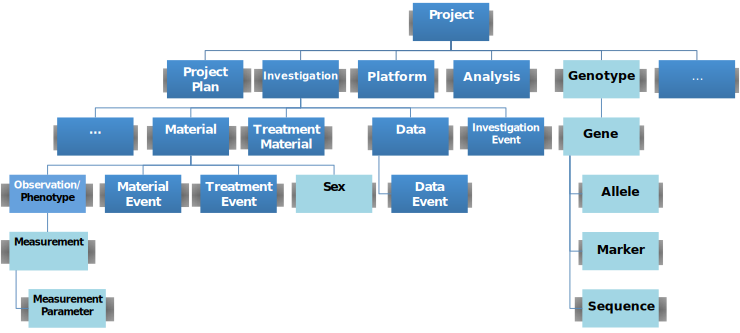
\includegraphics[
width=\paperwidth,
height=\paperheight,
keepaspectratio=true
]{podd_ont.png}}
\begin{frame}[plain]{}
% \frametitle{Phenomics ontology for PODD}
% \invisible

% \begin{center}
 % podd_ont.pdf: 720x540 pixel, 72dpi, 25.40x19.05 cm, bb=0 0 720 540
\end{frame}
\egroup

\begin{frame}
\frametitle{Demo} 

\end{frame}

\begin{frame}
\frametitle{Evaluation}

\end{frame}

\begin{frame}
\frametitle{Next steps}

\end{frame}


\begin{frame}
\frametitle{Questions}

Open source code can be found online at:

\url{https://github.com/podd}

My email is: peter.ansell@uq.edu.au

\end{frame}

\end{document}


